\chapter{Resultados y discusión}
\label{chap:resultados}
% Integración basada en main 9558099, campaña f395570, EF-01-C2 y OE3-C1.
% Las filas numéricas se generan desde fuentes conservadas en evidencias_redaccion/.

Este capítulo presenta los resultados del estudio computacional y examina su relación con los objetivos planteados. La exposición sigue la secuencia del capítulo~\ref{chap:metodologia}: primero se describe el conjunto sintético y sus controles; después se compara la recuperación de imágenes al 5\,\% de los conteos; finalmente se analiza la evaluación multifracción, el comportamiento local de las anomalías y el factor de reducción definido para el tercer objetivo. Los resultados corresponden al experimento concluido y a sus revisiones conservadas en el repositorio~\parencite{repositorioMuografia2026}.

La comparación distingue similitud de imagen, conservación de cuentas e interpretación física. SSIM y PSNR se calcularon en la representación transformada; el sesgo y los errores regionales se calcularon después de recuperar cuentas. Por ello, la mejora de una métrica no se utiliza como sustituto de las demás. Las cifras de prueba resumen tres geometrías con igual peso, mientras que generalización describe un único escenario y se informa por separado. Las veinte realizaciones por vista caracterizan el submuestreo de una referencia común; no aumentan el número de escenarios independientes.

\section{Conjunto sintético y controles de la campaña}\label{sec:res-oe1}
\subsection{Producto obtenido y diversidad de las referencias}
La campaña corregida produjo 114 imágenes de referencia, correspondientes a diecinueve geometrías y seis vistas por geometría. Cada imagen contiene $256\times256$ conteos direccionales. Se procesaron 1\,026 bloques, con 344 millones de primarios por vista y 39\,216 millones en toda la campaña. Estas cantidades describen los muones generados y transportados, no el total registrado en los píxeles, que dependió de cada escenario y de las condiciones de selección.

A partir de esas referencias se obtuvieron 9\,120 pares mediante submuestreo binomial, con cuatro fracciones y veinte realizaciones por fracción. Se conservaron 5\,760 pares de entrenamiento, 1\,440 de validación, 1\,440 de prueba y 480 de generalización en el conjunto completo. Para los entrenamientos al 5\,\% se utilizaron únicamente 1\,440 pares de entrenamiento y 360 de validación, conforme a la Tabla~\ref{tab:met-particiones}. Esta diferencia evita atribuir a cada modelo el uso de todas las estadísticas disponibles.

La Figura~\ref{fig:res-referencias} reúne configuraciones del catálogo y vistas con distinta suficiencia de conteo. La comparación permite observar la silueta proyectada del edificio y la dependencia angular del conteo. Su propósito es ilustrar la variación del conjunto, sin presentar la selección como muestra estadística de volcanes reales.
\FiguraPendienteMet{res_01_referencias_vector}{Referencias del conjunto corregido en escenarios y vistas seleccionados.}{fig:res-referencias}{Reexportar la figura 01-referencias del cierre OE1 desde sus matrices originales, usando celdas vectoriales. Conservar exactamente los seis casos de datos-figuras.json: geo-train-01 vista 0, geo-train-06 vista 3, geo-test-03 vista 5, geo-gen-01 vista 0, geo-val-01 vista 0 y geo-train-09 vista 1. Verificar la lista contra selected\_examples antes de dibujar. Organizar dos filas por tres columnas; indicar geometría y vista en cada panel. Mantener acimut y elevación en grados y una escala común de conteos, logarítmica y lineal entre cero y una cuenta. No usar una escala independiente por panel ni normalización de la red. No pegar los PNG del repositorio dentro de un PDF. Conservar las vistas bajo la meta de roca y declarar su selección. Fuente: objetivo-1/figuras/cierre-2026-10-03/datos-figuras.json y herramienta figuras\_cierre\_oe1.py.}

La reducción del conteo se aprecia en la Figura~\ref{fig:met-pares}, que conserva una misma vista y la misma escala para las cuatro fracciones. Al disminuir el número de eventos se incrementa la fluctuación relativa y aparecen más celdas vacías en las regiones de baja transmisión. Las entradas reducidas proceden de la referencia finita; no son simulaciones de transporte independientes. En consecuencia, el conjunto permite estudiar recuperación condicionada por ese mecanismo de reducción, con una referencia que conserva su propia incertidumbre de conteo.

\subsection{Respuesta en los bordes angulares}
Las 1\,710 regiones de borde cumplieron el criterio establecido antes de la campaña. La Figura~\ref{fig:res-bordes} representa las diferencias respecto del interior y los intervalos simultáneos, junto con la tolerancia de un punto porcentual. El cumplimiento se refiere al intervalo completo, según la Ecuación~\eqref{eq:met-aceptacion}, y no solo a que las estimaciones puntuales se aproximen a cero.
\begin{figure}[htbp]\centering
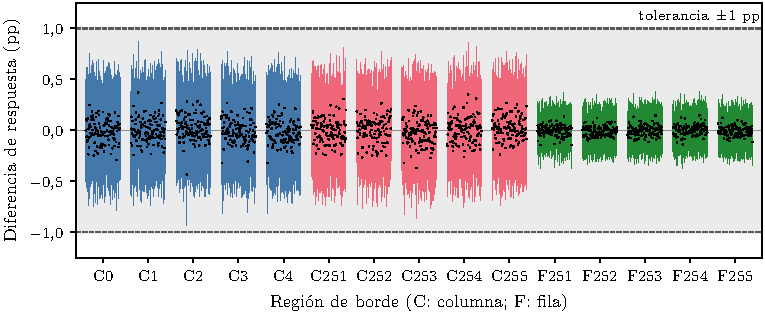
\includegraphics[width=\linewidth]{res_02_bordes.pdf}
\caption[Control de respuesta en bordes angulares]{Diferencias de respuesta de las quince regiones de borde en las 114 vistas, expresadas en puntos porcentuales. C identifica columnas y F filas; las líneas discontinuas delimitan la tolerancia de $\pm1$ punto porcentual. Los intervalos corresponden al control simultáneo de la campaña. Fuente: elaboración de los autores a partir de la evaluación congelada del OE1.}\label{fig:res-bordes}
\end{figure}

Este resultado respalda la estabilidad del observable en los extremos de la ventana respecto del interior definido por la misma fuente. Su alcance es específico: no verifica por sí mismo una respuesta instrumental, la calibración del flujo ni la equivalencia entre el plano computacional y un detector físico. La referencia ideal utilizada en el control responde a las hipótesis de generación; por tanto, superar esta comprobación no elimina las simplificaciones de la fuente y del transporte.

\subsection{Suficiencia de conteo en roca y conservación de excepciones}
En las 21\,816 regiones de roca de $4\times4$ píxeles se encontraron 20\,713 con al menos cien cuentas, equivalentes al 94,944\,\% del total. Sin embargo, el criterio se había definido por vista: al menos el 90\,\% de sus regiones debía alcanzar ese conteo. La meta se cumplió en 107 de las 114 vistas. Las siete restantes se conservaron y se identifican en la Tabla~\ref{tab:res-roca}; no se retiraron para mejorar el porcentaje global.
\begin{table}[htbp]\centering\small
\caption[Vistas bajo la meta descriptiva de roca]{Vistas que no alcanzaron el 90\,\% de regiones de roca con cien cuentas. Se conservaron en el conjunto definitivo. Fuente: registros de calidad del OE1.}\label{tab:res-roca}
\begin{tabular}{@{}lrrrr@{}}\toprule
Geometría & Vista & ROI conformes & ROI totales & Proporción (\%)\\\midrule
% Filas generadas desde tablas/res_roca_filas.tex
\texttt{geo-test-03} & 1 & 199 & 222 & 89{,}64\\
\texttt{geo-test-03} & 5 & 198 & 222 & 89{,}19\\
\texttt{geo-train-06} & 3 & 218 & 244 & 89{,}34\\
\texttt{geo-train-09} & 1 & 185 & 206 & 89{,}81\\
\texttt{geo-train-09} & 4 & 185 & 206 & 89{,}81\\
\texttt{geo-train-09} & 5 & 184 & 206 & 89{,}32\\
\texttt{geo-train-12} & 2 & 210 & 234 & 89{,}74\\
\bottomrule\end{tabular}\end{table}

Las proporciones de estas vistas quedaron entre 89,19 y 89,81\,\%. La Figura~\ref{fig:res-roca} sitúa las excepciones dentro del conjunto completo, evitando que el agregado oculte su distribución. La diferencia frente a la meta fue pequeña, pero se conserva como incumplimiento de ese indicador descriptivo y no como una aprobación redondeada.
\FiguraPendienteMet{res_03_roca_vector}{Suficiencia de conteo en roca por geometría y vista.}{fig:res-roca}{Adaptar la figura de calidad de roca del cierre OE1 o fig4-3\_roca de los estudiantes. Crear mapa de 19 filas por seis vistas con F en porcentaje y marcar las siete excepciones de la Tabla de vistas bajo la meta. Dibujar las celdas como rectángulos vectoriales, con números legibles y umbral del 90 por ciento explícito. En un segundo panel mostrar proporción conforme frente al número de ROI de cada vista, para distinguir proporción y tamaño del soporte. No inferir precisión por píxel de la suma en ROI. Fuente: datos-figuras-oe1.json, conservado en evidencias\_redaccion, campos metrics, roi, roi\_ge100 y fraction\_ge100. Verificar 114 vistas y 7 excepciones. Mantener datos y criterios; no ejecutar nueva simulación.}

El umbral de cien cuentas se aplicó a la suma de dieciséis píxeles. No permite afirmar que cada píxel tenga cien eventos ni que toda la imagen alcance una precisión relativa del 10\,\%. Además, las regiones fueron seleccionadas mediante la columna nominal del cono homogéneo. El indicador describe la disponibilidad de conteo en ese soporte y no sustituye una evaluación de contraste de todas las anomalías.

\subsection{Integridad, reproducción y alcance del primer objetivo}
La revisión verificó 477 huellas de los productos de fusión y exportación y reprodujo los 9\,120 pares, con coincidencia de las 342 huellas de contenido de sus arreglos. Se contrastaron las imágenes con los histogramas y se comprobó la conservación de cuentas y coordenadas. La distribución del conjunto también fue recuperada y verificada de manera independiente. Estas comprobaciones respaldan la identidad de los datos entregados y la reproducción de su posproceso.

No se realizó una segunda campaña independiente de transporte Geant4. La evidencia de esa etapa quedó constituida por la receta, las semillas, los bloques y sus registros. Esta distinción es relevante porque reproducir el submuestreo o verificar un archivo no equivale a reproducir todas las interacciones físicas que originaron la referencia.

El producto obtenido satisface el alcance idealizado adoptado para el OE1: un conjunto de imágenes de transmisión sintéticas, con distintas configuraciones y estadísticas de conteo. La representación cubre caminos de diferente columna de masa y contrastes de densidad, pero no caracteriza un volcán particular ni una población geológica. El cierre del objetivo conservó la fuente híbrida, el transporte de primarios, la exposición convencional y las siete excepciones de roca como condiciones de interpretación.

\section{Recuperación de imágenes al cinco por ciento}\label{sec:res-oe2}
\subsection{Modelos seleccionados y resultado de similitud}
El piloto concluyó tras doce épocas para U-Net y trece para cGAN. En ambos modelos, el mayor SSIM de validación correspondió a la época cinco, cuyos pesos se conservaron para la evaluación final. Las seis variantes E1 se obtuvieron mediante cinco épocas adicionales desde la cGAN original, manteniendo la última época de cada continuación de acuerdo con el diseño. Por tanto, los ocho modelos representan dos entrenamientos originales y seis continuaciones, no ocho ejecuciones independientes desde cero.

La Tabla~\ref{tab:res-f05} presenta todos los modelos y el comparador sin red al 5\,\%. Los valores de $Q$ se expresan en porcentaje; en las fuentes numéricas se almacenan como fracciones. SSIM y PSNR aumentan con la similitud en la representación transformada, mientras que un $Q$ menor indica menor sesgo regional agregado.
\begin{table}[htbp]\centering\small
\caption[Evaluación de todos los modelos al 5\,\%]{Similitud y sesgo regional al 5\,\% de conteos. Prueba resume tres geometrías con igual peso y generalización corresponde a una. Fuente: síntesis auditada del complemento, consistente con EF-01-C2 en estas métricas.}\label{tab:res-f05}
\begin{tabular}{@{}lrrr@{}}\toprule
Método & SSIM & PSNR (dB) & $Q$ (\%)\\\midrule
% Filas generadas desde tablas/res_f05_filas.tex
\multicolumn{4}{l}{\textit{Prueba}}\\
Entrada sin red & 0{,}7643 & 24{,}258 & 1{,}832\\
U-Net original & 0{,}8545 & 33{,}074 & 22{,}388\\
cGAN original & 0{,}8342 & 31{,}170 & 14{,}566\\
B1--C0 & 0{,}8277 & 30{,}839 & 5{,}825\\
B1--C1 & 0{,}8278 & 30{,}849 & 4{,}821\\
B2--C0 & 0{,}8274 & 30{,}772 & 3{,}996\\
B2--C1 & 0{,}8273 & 30{,}770 & 4{,}727\\
B3--C0 & 0{,}8263 & 30{,}729 & 4{,}828\\
B3--C1 & 0{,}8273 & 30{,}768 & 5{,}480\\
\midrule
\multicolumn{4}{l}{\textit{Generalización}}\\
Entrada sin red & 0{,}7502 & 23{,}904 & 1{,}093\\
U-Net original & 0{,}8454 & 32{,}883 & 26{,}505\\
cGAN original & 0{,}8252 & 31{,}047 & 16{,}959\\
B1--C0 & 0{,}8161 & 30{,}485 & 3{,}808\\
B1--C1 & 0{,}8151 & 30{,}509 & 4{,}323\\
B2--C0 & 0{,}8145 & 30{,}331 & 4{,}131\\
B2--C1 & 0{,}8154 & 30{,}403 & 4{,}755\\
B3--C0 & 0{,}8149 & 30{,}404 & 4{,}054\\
B3--C1 & 0{,}8146 & 30{,}371 & 2{,}271\\
\bottomrule\end{tabular}\end{table}

En prueba, la cGAN incrementó el SSIM de 0,7643 a 0,8342 y el PSNR de 24,258 a 31,170~dB respecto de la entrada. La U-Net obtuvo valores mayores, de 0,8545 y 33,074~dB. El mismo orden se observó en generalización: U-Net superó a cGAN en ambas métricas, y las dos redes superaron la entrada. Bajo las configuraciones evaluadas, la componente adversaria no proporcionó una ventaja global de SSIM o PSNR frente al generador entrenado únicamente con L1.

La comparación visual de la Figura~\ref{fig:res-comparacion} complementa esas cifras con casos fijados por índice. Se mantiene la misma vista y realización en cada geometría y una escala común de la transformación, para evitar que cambios de contraste gráfico se confundan con diferencias entre métodos.
\FiguraPendienteMet{res_06_comparacion_vector}{Comparación de referencia, entrada al 5\,\% y modelos originales en casos fijados por índice. Todas las geometrías corresponden a vista 0 y realización 0, con una escala común de representación.}{fig:res-comparacion}{Recuperar la composición fig4-7\_comparacion\_fija de los estudiantes, sin cambiar la selección. Cuatro filas: geo-test-01, geo-test-02, geo-test-03 y geo-gen-01; cuatro columnas: referencia, entrada al 5 por ciento, U-Net y cGAN. Usar vista 0 y realización 0 en todas las geometrías. Fuente editable: figuras-fuentes/resultados-estudiantes/figuras/fuentes/fig4-7\_comparacion\_fija.py y el paquete fuentes/datos\_figuras/cortes\_oe2.npz del mismo directorio de resultados estudiantiles; verificar las huellas de procedencia conservadas antes de usarlo. Representar las 256 por 256 celdas sin interpolación como polígonos vectoriales; sustituir imshow por un trazado vectorial equivalente y evitar rasterized. Escala T común de 0 a 0,52, barra única, acimut y elevación en grados tomados de las coordenadas. Separar visualmente generalización. No reajustar escalas por modelo ni seleccionar las imágenes de mejor SSIM. Guardar el PDF y su fuente editable.}

La apariencia más regular de una salida puede ser consistente con un incremento de similitud, pero no demuestra por sí sola recuperación del contenido físico. SSIM y PSNR comparan cada imagen con la misma referencia finita. Además, se calculan después de una transformación no lineal que comprime el intervalo de conteos; una discrepancia pequeña en ese dominio puede traducirse en una diferencia relevante al recuperar cuentas.

\subsection{Compromiso entre similitud y conservación regional}
La mejora de SSIM y PSNR coexistió con un aumento del sesgo regional. En prueba, $Q$ pasó de 1,832\,\% en la entrada a 14,566\,\% con cGAN y 22,388\,\% con U-Net. En generalización pasó de 1,093\,\% a 16,959 y 26,505\,\%, respectivamente. La Figura~\ref{fig:res-compromiso} permite examinar conjuntamente esos indicadores; un desplazamiento hacia mayor similitud no implica necesariamente acercamiento a menor sesgo.
\begin{figure}[htbp]\centering
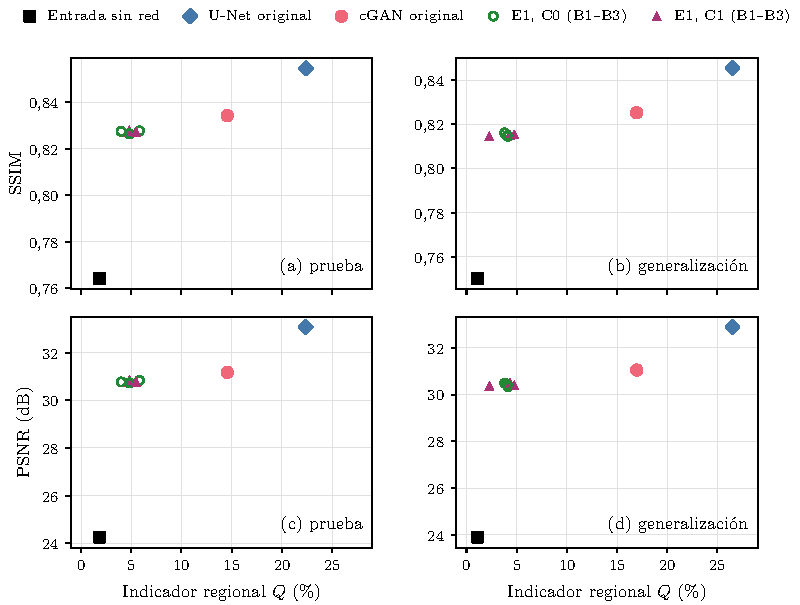
\includegraphics[width=\linewidth]{res_04_compromiso.pdf}
\caption[Similitud frente a sesgo regional al 5\,\%]{Relación de SSIM y PSNR con $Q$ al 5\,\%, para prueba y generalización por separado. Se conservan las seis continuaciones E1; cada punto representa el resumen de una configuración, no una repetición independiente. Fuente: elaboración de los autores a partir de los resultados EF-01-C2.}\label{fig:res-compromiso}
\end{figure}

La entrada escalada conserva en esperanza condicional las cuentas de la referencia bajo el mecanismo binomial. Ese atributo explica que pueda mantener promedios regionales cercanos a la referencia aun cuando exhiba mayor ruido por píxel. Las redes optimizaron pérdidas que combinan discrepancia transformada y, en la cGAN, una puntuación adversaria. Ninguna de esas pérdidas originales impuso conservación exacta de las cuentas de cada región. Esta diferencia entre lo optimizado y lo evaluado es compatible con el compromiso observado, aunque el experimento no identifica una causa única de todos los sesgos.

Las continuaciones E1 redujeron $Q$ respecto de las redes originales: en prueba sus valores quedaron entre 3,996 y 5,825\,\%, con SSIM entre 0,8263 y 0,8278. Persistió, sin embargo, un sesgo superior al de la entrada. La mejora regional se obtuvo junto con una similitud menor que la de U-Net y cGAN originales. No corresponde seleccionar retrospectivamente el menor $Q$ de una semilla y presentarlo como resultado universal del método.

El indicador $Q$ aplica valor absoluto después de promediar sesgos entre realizaciones, según la Ecuación~\eqref{eq:met-q}. Por tanto, no debe interpretarse como error medio absoluto de todos los píxeles ni como error porcentual de densidad. Sus diferencias se complementan con error espacial y contraste, porque una suma regional cercana a la referencia puede ocultar redistribución interna de cuentas.

\subsection{Efecto de la pérdida espacial de borde}
La Figura~\ref{fig:res-borde} compara los errores de borde de las tres parejas E1. La variante C1 añade el término espacial al término regional ya presente en C0. La Tabla~\ref{tab:res-borde} cuantifica la diferencia para cada geometría, calculando la reducción relativa como cien veces uno menos el cociente entre el error C1 y el error C0.
\begin{figure}[htbp]\centering
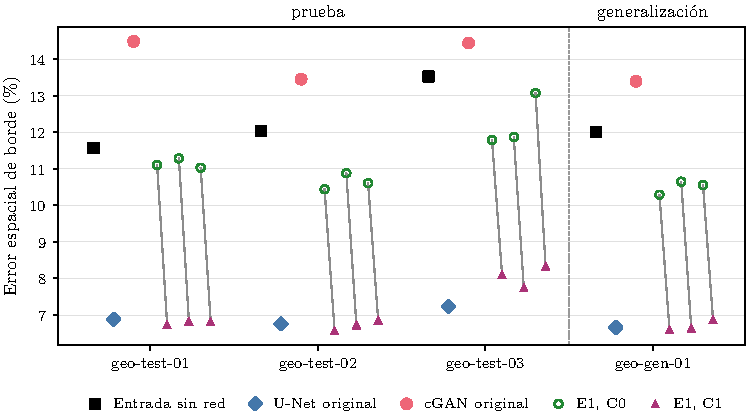
\includegraphics[width=\linewidth]{res_05_borde.pdf}
\caption[Error espacial de borde por geometría]{Error de borde al 5\,\% en las cuatro geometrías reservadas. Los segmentos unen C0 y C1 de una misma pareja; los puntos de una geometría no representan réplicas independientes. Se distinguen prueba y generalización. Fuente: elaboración de los autores a partir de EF-01-C2.}\label{fig:res-borde}
\end{figure}
\begin{table}[htbp]\centering\small
\caption[Comparación pareada del error de borde]{Error espacial de borde en porcentaje y reducción relativa de C1 respecto de C0. Fuente: recálculo desde los resúmenes por geometría de EF-01-C2.}\label{tab:res-borde}
\begin{tabular}{@{}llrrr@{}}\toprule
Geometría & Pareja & C0 (\%) & C1 (\%) & Reducción (\%)\\\midrule
% Filas generadas desde tablas/res_borde_filas.tex
\texttt{geo-test-01} & B1 & 11{,}103 & 6{,}737 & 39{,}33\\
\texttt{geo-test-01} & B2 & 11{,}286 & 6{,}830 & 39{,}49\\
\texttt{geo-test-01} & B3 & 11{,}029 & 6{,}819 & 38{,}17\\
\texttt{geo-test-02} & B1 & 10{,}442 & 6{,}569 & 37{,}10\\
\texttt{geo-test-02} & B2 & 10{,}882 & 6{,}731 & 38{,}15\\
\texttt{geo-test-02} & B3 & 10{,}607 & 6{,}865 & 35{,}27\\
\texttt{geo-test-03} & B1 & 11{,}791 & 8{,}105 & 31{,}26\\
\texttt{geo-test-03} & B2 & 11{,}871 & 7{,}750 & 34{,}72\\
\texttt{geo-test-03} & B3 & 13{,}075 & 8{,}339 & 36{,}22\\
\texttt{geo-gen-01} & B1 & 10{,}291 & 6{,}604 & 35{,}83\\
\texttt{geo-gen-01} & B2 & 10{,}649 & 6{,}647 & 37{,}58\\
\texttt{geo-gen-01} & B3 & 10{,}552 & 6{,}880 & 34{,}80\\
\bottomrule\end{tabular}\end{table}

C1 redujo el error de borde en las doce comparaciones pareja--geometría, entre 31,26 y 39,49\,\%. El efecto es coherente con la incorporación de una pérdida que actúa explícitamente sobre esa franja. No obstante, restringir el error de borde no garantiza corregir el interior ni mejorar simultáneamente la similitud y el contraste. Las diferencias de $Q$ entre C0 y C1 cambiaron según pareja y geometría, lo que impide describir C1 como superior en todos los aspectos.

Las doce comparaciones predeclaradas de EF-01, seis por partición, conservaron la clasificación descriptiva de compromiso o deterioro en al menos un indicador. Esa clasificación no expresa significación estadística. Las parejas comparten pesos iniciales y el catálogo reservado tuvo exposición histórica; la evidencia se refiere al comportamiento de las configuraciones y escenas evaluadas.

\section{Transferencia de los modelos a otras fracciones}\label{sec:res-oe3}
\subsection{Evaluación completa y correspondencia entre entregas}
El complemento OE3-C1 añadió 96 matrices con 11\,520 predicciones, correspondientes a los ocho modelos, las tres fracciones nuevas y las cuatro geometrías. Junto con las 3\,840 salidas al 5\,\% conservadas de EF-01, se evaluaron 15\,360 predicciones. Las redes mantuvieron los pesos ajustados al 5\,\%, por lo que el resultado describe transferencia entre estadísticas y no entrenamiento especializado para cada nivel de conteo.

La revisión verificó los 294 archivos del manifiesto y las 96 matrices nuevas, con aproximadamente 3,02~GB de datos binarios. El recálculo de tablas y registros numéricos coincidió dentro de la tolerancia establecida entre entornos, con una diferencia absoluta máxima de $7{,}105\times10^{-15}$. Esta concordancia respalda la reproducción del cálculo de métricas sobre predicciones conservadas; no se presenta como una repetición local de toda la inferencia GPU ni de los entrenamientos.

\subsection{Respuesta de la cGAN frente a la estadística de entrada}
La Tabla~\ref{tab:res-multifraccion} compara la cGAN original y la entrada sin red en las cuatro fracciones. Se incluye el comparador de cada fracción para que el desempeño de la red pueda examinarse frente a la información disponible en su propia entrada, además del referente fijo utilizado para el factor de reducción.
\begin{table}[htbp]\centering\small
\caption[cGAN y entrada sin red en cuatro fracciones]{Evaluación de la cGAN original y de la entrada sin red en las cuatro fracciones. Se conservan los mismos pesos entrenados al 5\,\%. Fuente: síntesis auditada OE3-C1.}\label{tab:res-multifraccion}
\begin{tabular}{@{}rlrrr@{}}\toprule
Fracción & Método & SSIM & PSNR (dB) & $Q$ (\%)\\\midrule
% Filas generadas desde tablas/res_multifraccion_filas.tex
\multicolumn{5}{l}{\textit{Prueba}}\\
1\,\% & Entrada sin red & 0{,}6959 & 22{,}537 & 2{,}897\\
1\,\% & cGAN original & 0{,}8124 & 29{,}264 & 45{,}279\\
5\,\% & Entrada sin red & 0{,}7643 & 24{,}258 & 1{,}832\\
5\,\% & cGAN original & 0{,}8342 & 31{,}170 & 14{,}566\\
10\,\% & Entrada sin red & 0{,}7964 & 25{,}722 & 1{,}334\\
10\,\% & cGAN original & 0{,}8378 & 31{,}213 & 15{,}732\\
50\,\% & Entrada sin red & 0{,}9250 & 33{,}101 & 0{,}437\\
50\,\% & cGAN original & 0{,}7761 & 27{,}255 & 38{,}996\\
\midrule
\multicolumn{5}{l}{\textit{Generalización}}\\
1\,\% & Entrada sin red & 0{,}6851 & 22{,}299 & 3{,}067\\
1\,\% & cGAN original & 0{,}8040 & 29{,}069 & 52{,}203\\
5\,\% & Entrada sin red & 0{,}7502 & 23{,}904 & 1{,}093\\
5\,\% & cGAN original & 0{,}8252 & 31{,}047 & 16{,}959\\
10\,\% & Entrada sin red & 0{,}7834 & 25{,}349 & 0{,}895\\
10\,\% & cGAN original & 0{,}8304 & 31{,}174 & 10{,}179\\
50\,\% & Entrada sin red & 0{,}9197 & 32{,}752 & 0{,}449\\
50\,\% & cGAN original & 0{,}7644 & 27{,}274 & 29{,}066\\
\bottomrule\end{tabular}\end{table}

En prueba, la cGAN obtuvo SSIM de 0,8124 al 1\,\%, 0,8342 al 5\,\% y 0,8378 al 10\,\%. El PSNR pasó de 29,264 a 31,170 y 31,213~dB en esos niveles. El incremento entre 5 y 10\,\% fue pequeño frente al cambio de conteos. Al 50\,\%, el SSIM descendió a 0,7761 y el PSNR a 27,255~dB, por debajo de la entrada sin red con esa fracción. En generalización se observó el mismo deterioro de similitud al 50\,\%.

El sesgo regional tampoco siguió una reducción uniforme con el conteo. En prueba, $Q$ fue 45,279\,\% al 1\,\%, 14,566\,\% al 5\,\%, 15,732\,\% al 10\,\% y 38,996\,\% al 50\,\%. Una entrada con más eventos no aseguró mejor salida de una red entrenada con otra estadística. El escalamiento por la fracción mantiene la esperanza condicional de cuentas, pero no iguala la distribución de fluctuaciones ni convierte el entrenamiento al 5\,\% en entrenamiento para todas las entradas.

La Figura~\ref{fig:res-multifraccion} debe leerse junto con la tabla para identificar los cambios de cada modelo sin suponer monotonía. Las ocho redes presentaron menor SSIM y PSNR al 50\,\% que al 5\,\% y que la entrada sin red al 50\,\%, en ambas particiones. Se conserva el conjunto completo de 72 filas de la síntesis en el material numérico asociado al manuscrito, sin excluir variantes desfavorables.
\FiguraPendienteMet{res_07_multifraccion_vector}{Similitud y sesgo regional en cuatro fracciones de conteo, para prueba y generalización. Se conservan los ocho modelos y la entrada sin red. Todas las redes se entrenaron al 5\,\%; las líneas unen puntos evaluados como guía visual.}{fig:res-multifraccion}{Elaborar seis paneles: SSIM, PSNR y Q en columnas; prueba y generalización en filas. Fuente única: evidencias\_redaccion/sintesis\_metricas.csv, 72 filas, cuatro fracciones y nueve métodos. Dibujar entrada, U-Net y cGAN con estilos distinguibles; conservar las seis continuaciones con líneas finas y leyenda B1--B3/C0--C1, sin promediar semillas ni elegir la mejor. Eje horizontal: 1, 5, 10 y 50 por ciento, preferiblemente logarítmico con esas marcas. Convertir Q de fracción a porcentaje solo al representar. Unir puntos como guía visual; no interpolar factores. Indicar que todas las redes fueron entrenadas al 5 por ciento. Reemplazar fig4-6\_curvas\_exposicion, que solo representa las redes al 5 por ciento. Los promedios de estas curvas no sustituyen el criterio por vista. Exportar líneas, símbolos y textos vectoriales y conservar script.}

Este comportamiento acota la aplicabilidad de los pesos obtenidos. Es compatible con una dependencia del modelo respecto de la estadística utilizada durante el ajuste, pero no demuestra por sí mismo qué mecanismo interno produjo el deterioro. Tampoco implica que una red entrenada específicamente al 50\,\% o con varias fracciones reprodujera el mismo resultado. El experimento permite describir el comportamiento observado; una explicación causal requeriría un diseño adicional que no forma parte del estudio cerrado.

\section{Conservación de anomalías y métricas locales}\label{sec:res-locales}
\subsection{Soportes y lectura conjunta de los indicadores}
La evaluación local se realizó sobre regiones y controles definidos geométricamente, sin seleccionar anomalías por el resultado de la red. En el soporte común multifracción se conservaron diecinueve combinaciones anomalía--vista de prueba y once de generalización para SNR. CNR y contraste utilizaron veintiuna y once, respectivamente. Los casos no estimables permanecieron identificados y no se sustituyeron por ceros.

La Tabla~\ref{tab:res-locales} compara la entrada y la cGAN al 5\,\%. Se presentan errores absolutos respecto de la referencia y proporciones de inversión de signo, siguiendo el orden de agregación de la sección~\ref{subsec:met-locales}. Cada error se calcula por realización antes de resumir casos y geometrías. Por ello, los valores de contraste de esta tabla no son intercambiables con el resumen histórico C2.
\begin{table}[htbp]\centering\small
\caption[Errores locales de entrada y cGAN al 5\,\%]{Errores absolutos de indicadores locales y proporción de inversiones de signo del contraste al 5\,\%. Los tres errores son adimensionales y la última columna se expresa en porcentaje. Fuente: soporte común de la síntesis OE3-C1.}\label{tab:res-locales}
\begin{tabular}{@{}lrrrr@{}}\toprule
Método & Error SNR & Error CNR & Error contraste & Inversión (\%)\\\midrule
% Filas generadas desde tablas/res_locales_filas.tex
\multicolumn{5}{l}{\textit{Prueba}}\\
Entrada sin red & 0{,}6497 & 0{,}0567 & 0{,}1707 & 38{,}12\\
cGAN original & 0{,}1804 & 0{,}0646 & 0{,}0756 & 43{,}54\\
\midrule
\multicolumn{5}{l}{\textit{Generalización}}\\
Entrada sin red & 0{,}6509 & 0{,}0709 & 0{,}1588 & 40{,}00\\
cGAN original & 0{,}0972 & 0{,}0825 & 0{,}0786 & 44{,}09\\
\bottomrule\end{tabular}\end{table}

En prueba, el error de SNR espacial disminuyó de 0,6497 a 0,1804 y el error de contraste de 0,1707 a 0,0756. Simultáneamente, el error de CNR aumentó de 0,0567 a 0,0646 y la proporción de inversión de signo pasó de 38,12 a 43,54\,\%. En generalización se observó el mismo sentido de cambio: menores errores de SNR y contraste, junto con mayor error de CNR y mayor inversión de signo.

Los indicadores, por tanto, no sostienen una mejora uniforme de la información local. Reducir el error medio de un cociente no garantiza preservar su signo en todos los casos. Una predicción próxima a cero puede reducir una discrepancia grande y, a la vez, cruzar el signo de una referencia pequeña. Además, la referencia conserva fluctuación de conteo, de modo que su signo es sensible en anomalías con contraste cercano a cero. Esta limitación se mantuvo sin eliminar retrospectivamente esos casos mediante un umbral favorable.

\subsection{Suavizado, señal local y límites de detectabilidad}
La reducción de dispersión espacial puede incrementar SNR y regularizar visualmente la imagen. Sin embargo, la dispersión incluye tanto ruido como estructura. Una salida más uniforme puede atenuar una anomalía o modificar su relación con el fondo. El CNR firmado aporta otra perspectiva porque conserva la diferencia entre la media objetivo y la media de controles, relativa a la dispersión de esos controles.

Estas métricas se definieron para estudiar el conjunto sintético y no como probabilidades de detección. La geometría de las anomalías era conocida y se utilizó para construir máscaras; en una aplicación a un volcán real esa información no estaría disponible necesariamente. En consecuencia, los resultados evalúan preservación en regiones predefinidas, sin demostrar localización autónoma de estructuras desconocidas.

El descenso del error de contraste tampoco puede presentarse como reconstrucción de densidad. El contraste comparó cuentas entre rayos de longitudes próximas y a igual elevación, conservando diferencias geométricas y una referencia finita. La mejora de ese indicador es un resultado específico que debe leerse junto con $Q$, error espacial y CNR. La coexistencia de mejoras y deterioros constituye el hallazgo, en lugar de un motivo para escoger una única métrica como resumen favorable.

\section{Factor de reducción y diagnóstico de opacidad}\label{sec:res-factor}
\subsection{Resultado del criterio operativo por vista}
El criterio de la sección~\ref{subsec:met-minimo} exigió alcanzar simultáneamente SSIM y PSNR del referente sin red al 50\,\% en todas las vistas de cada partición. Las 768 combinaciones modelo--fracción--vista se conservaron en la evaluación: ocho modelos, cuatro fracciones y veinticuatro vistas. Ninguna satisfizo conjuntamente ambas condiciones. La Tabla~\ref{tab:res-benchmark} muestra el balance por modelo y partición.
\begin{table}[htbp]\centering\small
\caption[Balance del criterio conjunto por vista]{Combinaciones fracción--vista que alcanzaron conjuntamente SSIM y PSNR del referente al 50\,\%. Cada modelo tiene 72 comparaciones en prueba y 24 en generalización. El mínimo y el factor no se determinaron en ninguna partición. Fuente: registro auditado de 768 comparaciones OE3-C1.}\label{tab:res-benchmark}
\begin{tabular}{@{}lrrl@{}}\toprule
Modelo & Prueba & Generalización & $f_{\min}$ y $R$\\\midrule
% Filas generadas desde tablas/res_benchmark_filas.tex
U-Net original & 0/72 & 0/24 & No determinado\\
cGAN original & 0/72 & 0/24 & No determinado\\
B1--C0 & 0/72 & 0/24 & No determinado\\
B1--C1 & 0/72 & 0/24 & No determinado\\
B2--C0 & 0/72 & 0/24 & No determinado\\
B2--C1 & 0/72 & 0/24 & No determinado\\
B3--C0 & 0/72 & 0/24 & No determinado\\
B3--C1 & 0/72 & 0/24 & No determinado\\
\bottomrule\end{tabular}\end{table}

Los conjuntos de aceptación definidos en la Ecuación~\eqref{eq:met-aceptadas} fueron vacíos. Por ello, no se obtuvo un mínimo de la rejilla ni el factor asociado de la Ecuación~\eqref{eq:met-factor}. El resultado se informa como no determinado o no demostrado bajo el criterio adoptado. No corresponde escribir que el factor fue cero, pues no se estimó una razón nula; tampoco fue uno, que habría requerido aceptar la fracción del 50\,\% sin reducción.

La ausencia de una fracción aceptada es un resultado experimental. El criterio no se cambió después para asegurar una cifra favorable, ni se interpoló entre los niveles disponibles. El alcance permanece ligado a estos modelos, estas fracciones y este referente. No demuestra que cualquier arquitectura, entrenamiento o conjunto futuro sea incapaz de reducir conteos con calidad útil.

\subsection{Comparación descriptiva con el doble de conteos}
La comparación secundaria de cGAN al 5\,\% frente a la entrada sin red al 10\,\% mantuvo una mejora de SSIM y PSNR en las veinticuatro vistas reservadas y en las 480 correspondencias por realización. Ambas imágenes se evaluaron frente a la misma referencia completa. La comparación describe una razón nominal de conteos 2:1; no mide directamente distancia entre la salida de la red y la entrada al 10\,\%.

En prueba, la entrada al 10\,\% presentó SSIM de 0,7964 y PSNR de 25,722~dB, frente a 0,8342 y 31,170~dB de cGAN al 5\,\%. El sesgo regional siguió el comportamiento contrario: $Q$ fue 1,334\,\% en esa entrada y 14,566\,\% en la cGAN. La ganancia de similitud no estuvo acompañada de mejor conservación regional.

La comparación 2:1 y el resultado negativo frente al 50\,\% son compatibles porque utilizan referentes diferentes. La primera documenta una mejora descriptiva de determinadas métricas; el segundo responde al criterio operativo del complemento. Ninguno permite presentar veinte veces menos conteos como reducción efectiva de adquisición con calidad equivalente. La relación entre conteos y tiempo sigue siendo idealizada, sin calibración de un instrumento de campo.

\subsection{Opacidad nominal y diferencia respecto de una inversión}
El diagnóstico geométrico conservó 54 registros de anomalía y vista, de los cuales 48 cumplieron el soporte C2. Se comprobaron unidades y composición mediante cuatro casos analíticos y se reprodujeron los registros geométricos. La descomposición de la Ecuación~\eqref{eq:met-opacidaddelta} presentó un residuo máximo de aproximadamente $1{,}0004\times10^{-10}$~g\,cm$^{-2}$, compatible con precisión numérica del cálculo.

En los registros elegibles, la contribución nominal de densidad varió entre $-17\,242{,}01$ y $+5\,616{,}20$~g\,cm$^{-2}$. El término debido a diferencia de longitud frente a los controles no cambió el signo de la contribución de densidad en esos casos. Estos valores describen el catálogo y los rayos seleccionados; no son errores de reconstrucción de una red ni umbrales de detección de anomalías.

La Figura~\ref{fig:res-opacidad} separa las contribuciones geométricas para facilitar su interpretación. Se conservaron las seis filas elegibles de la anomalía 2 de \texttt{geo-gen-01} con su advertencia de material: el catálogo declara 0,048~g\,cm$^{-3}$, mientras el constructor conservado utiliza aire para densidades inferiores a 0,05~g\,cm$^{-3}$. El diagnóstico no certificó la densidad efectiva de cada material del binario de producción.
\FiguraPendienteMet{res_08_opacidad_nominal}{Contribuciones nominales de densidad y longitud en los controles geométricos: 48 combinaciones elegibles de geometría, anomalía y vista. Los símbolos huecos identifican la advertencia de material de geo-gen-01, anomalía 2. Las seis combinaciones no elegibles se registran sin asignarles cero. No representa opacidad reconstruida por la red.}{fig:res-opacidad}{Usar evidencias\_redaccion/opacidad\_nominal.csv y las definiciones de OPACIDAD\_NOMINAL\_Y\_ALCANCE.md del repositorio. Para las 48 filas elegibles, representar por geometría, anomalía y vista el término de densidad, el término de diferencia de longitud y su suma; puede usarse un gráfico de puntos en tres paneles alineados con eje en g/cm cuadrado y línea de cero. Identificar sin ocultar las seis filas de geo-gen-01 anomalía 2 con trama o símbolo hueco y nota de densidad nominal distinta de material efectivo. Registrar aparte las seis filas no elegibles, sin asignar cero. Rotular claramente opacidad nominal del catálogo; no usar opacidad reconstruida ni error de la red. Conservar unidades, signos y valores exactos antes del redondeo. Exportar PDF vectorial con fuente editable.}

El contraste de cuentas es adimensional, mientras que la opacidad integra densidad y longitud. Calcular esta última desde una geometría conocida no demuestra que pueda recuperarse desde la imagen mejorada. No se ejecutó una inversión validada de las predicciones a opacidad. La inversión de opacidad se plantea como una extensión futura, no como un requisito adicional de los objetivos aprobados. El contraste no se interpretó como opacidad ni se atribuyó causalmente el desempeño de las redes a la discrepancia de material.

\section{Discusión integrada y alcance de los resultados}\label{sec:res-discusion}
\subsection{Correspondencia entre la tarea aprendida y la calidad evaluada}
El experimento mostró que una red puede aproximarse a una referencia en la escala utilizada para entrenar y conservar, al mismo tiempo, discrepancias relevantes en cuentas. U-Net alcanzó los mayores SSIM y PSNR al 5\,\%, pero también el mayor $Q$ entre los modelos originales. La cGAN presentó un compromiso diferente, sin dominar al control en todas las métricas. Las continuaciones redujeron parte del sesgo y el término espacial mejoró el borde, aunque ninguna configuración eliminó de forma conjunta todas las discrepancias.

Estos resultados hacen necesario precisar la expresión calidad comparable. Si se refiere a SSIM y PSNR frente a entradas de baja estadística, existe una mejora documentada. Si se exige el criterio conjunto frente al referente sin red al 50\,\%, no se obtuvo aceptación en la rejilla. Si se pretende conservación cuantitativa de cuentas, contraste y opacidad, las alteraciones regionales y la ausencia de inversión limitan esa afirmación. Las tres lecturas responden a preguntas distintas y se mantienen separadas.

La transformación acotada contribuye a explicar por qué los indicadores deben examinarse en más de un dominio: comprime los conteos y su inversa amplifica de manera no uniforme las discrepancias. Sin embargo, esta propiedad matemática no prueba por sí sola el origen de cada error observado. El análisis permite establecer coexistencia y límites, sin atribuir todos los efectos a un único componente de la arquitectura o de la pérdida.

\subsection{Dependencia de los datos y alcance de generalización}
El número de escenarios reservados fue pequeño: tres de prueba y uno de generalización. Las veinte realizaciones de una vista comparten referencia y las vistas comparten geometría. Por ello, las numerosas predicciones no constituyen miles de escenarios independientes. Los promedios y comparaciones describen este catálogo, sin estimar una tasa poblacional de generalización a volcanes.

Las escenas reservadas tuvieron exposición histórica durante etapas anteriores. Aunque los modelos finales se ajustaron con entrenamiento y validación, esa historia impide presentar la evaluación como confirmación completamente independiente. De igual forma, el criterio del complemento se estableció antes de las nuevas inferencias, pero después de conocer resultados previos. Su aplicación fue explícita y completa; su carácter posterior limita la fuerza de la inferencia, no convierte el resultado desfavorable en una actividad sin ejecutar.

Las referencias de alta estadística son finitas. El submuestreo comparte eventos con ellas y la verdad de comparación corresponde a esa realización sintética, no a una intensidad instrumental exacta. La evaluación conserva ese vínculo y no extrapola automáticamente la mejora a adquisiciones independientes o a observaciones reales con fondo, respuesta del detector y condiciones ambientales variables.

\subsection{Balance del experimento concluido}
La Tabla~\ref{tab:res-balance} relaciona los productos obtenidos con las afirmaciones que la evidencia permite sostener. El cierre operativo de los tres objetivos se distingue del alcance científico de sus conclusiones.
\begin{table}[!htbp]\centering\small
\caption{Balance de resultados y alcance de los tres objetivos.}\label{tab:res-balance}
\begin{tabularx}{\linewidth}{@{}p{1.5cm}>{\raggedright\arraybackslash}X>{\raggedright\arraybackslash}X@{}}\toprule
Objetivo & Resultado obtenido & Alcance sustentado\\\midrule
OE1 & Conjunto de 114 referencias y 9\,120 pares, con controles e integridad revisados. & Cumplido y cerrado dentro de la familia sintética idealizada; sin equivalencia instrumental.\\
OE2 & cGAN implementada y entrenada; comparación con U-Net y seis continuaciones; mejoras de similitud al 5\,\%. & Ejecución y evaluación concluidas. Calidad comparable respaldada parcialmente por persistencia de sesgos y compromisos.\\
OE3 & Evaluación de ocho modelos en cuatro fracciones; indicadores locales y criterio por vista aplicados. & Experimento concluido con factor no demostrado bajo el criterio adoptado; sin reconstrucción cuantitativa de opacidad.\\\bottomrule
\end{tabularx}\end{table}

La aportación del estudio comprende tanto los productos reproducibles como la delimitación de su utilidad. Se obtuvo una cadena verificable desde la simulación hasta la evaluación multifracción y se cuantificó la diferencia entre suavizar imágenes, aumentar similitud y preservar cantidades relevantes para la muografía. El resultado negativo del criterio principal y los comportamientos locales desfavorables se conservan como parte de esa evidencia.

\FloatBarrier
